\chapter{Frontend-Suche}

Diese Kapitel handelt von der Implementierung ElasticSearchs in das Dietrich-Online Projekt. Dabei soll zuerst einmal die Suche und die automatische Vervollständigung komplett übertragen werden. Danach sollen noch eine neue Suchart, welche mehr Felder umfasst, sowie eine Suche, welche darauf basiert, welche Autoren bei der vorherigen Suche das meiste geschrieben haben.

\section{Indexierung}

Um die Daten zu indexieren, wurde eine statische Code-Analyse durchgeführt, welche Daten alles im Frontend angezeigt wurden. Dafür wurde der gesamte Code zur Suche untersucht und alle Werte aufgeschrieben. Aufgrund dieser Basis wurde daraufhin ein Query gebaut, welche alle Daten an den Aggregat-Filter weiterreicht. Dabei wurde dieser angepasst und enthält nun auch eine String Konkatenation, welche zuvor bei der Anzeige ausgeführt wurde.

Der Index ist hierbei der aktuell Größte im Dietrich-Online Projekt mit rund 1.4 Millionen Einträgen. Diese Größe des Index beläuft sich auf 2.4 Gigabyte.

Diese Zahl wird sich allerdings verringern lassen, wenn mehr Regeln zu Indexierung eingebaut werden. Aktuell werden alle Spalten mit Text, die unter 256 Zeichen fallen einmal als Keyword und als Volltext indexiert \ref{elaVgl:index}.

Der Query enthielt nun 13 Joins. Diese Datenmenge konnte Logstash nicht verarbeiten und stürzte ab. Der RAM musste auf 4 Gigabyte erhöht werden, damit der Index ordentlich aufgebaut werden konnte.

Damit nun verschiedene Pipelines gleichzeitig arbeiten können, musste eine Datei zur Verwaltung der Pipelines angelegt werden. In dieser wurde definiert, dass von den vier verfügbaren Workern jeweils einer pro Pipeline zur Verfügung steht, damit die Aggregation richtig funktioniert.

Für die Auto-Vervollständigung mussten zudem noch einige neue Felder angelegt werden. Es gibt im Projekt für jede Suchart eine eigene Vervollständigung. Um dies auch im Index abzubilden, wurden diverse Vervollständigungs-Felder angelegt, welche zum Teil einzelne Felder oder Feldmengen durchsuchen. Diese Felder wurden dann mithilfe des Aggregat Filters befüllt. Ein Beispiel:

Artikeltitel und die dazugehörige Sigle werden in zwei unterschiedlichen Felder gespeichert, sollten allerdings für die Vervollständigung zusammengesetzt werden.
Dafür wird in dem Aggregationsfilter von Logstash definiert, dass das Feld zusammengebaut wird \ref{lst:stringConcat}. Nun wird daraus entstandene String in das Suggestions-Feld von ElasticSearch gegeben. ElasticSearch indexiert daraufhin des String so, dass jedes Wort zur Auto-Vervollständigung benutzt werden kann. Als Ausgabe erscheint dabei aber immer der vollständige String.

\begin{lstlisting}[language=PHP, frame=single, label={lst:stringConcat}] 
    map['artikel_titel_suggest'] ||= 
        '['+event.get('lemma_bezeichnung').to_s+']'
            +event.get('artikel_titel').to_s
\end{lstlisting}

Sollten aus einem Datensatz mehrere Felder indexiert werden, ist es möglich auch ein Array von Daten an ElasticSearch weiterzugeben.

\section{Integration}

Die Integration folgte demselben Muster, wie die der Lemma Administration. Ich möchte hier allerdings auf ein paar Unterschiede eingehen. 

\subsection{Paginierung}

Die bisherige Paginierung holte sich bis zu 1001 Ergebnisse aus der Datenbank und generierte daraufhin die Paginierung. Die Begrenzung ergibt sich daher, dass die vollen Datensätze aus der Datenbank geholt wurden, und dies bei größeren Zahlen zu einer langen Laufzeit führte.

Diese Einschränkung kann nun mit ElasticSearch entfernt werden. Dazu wird zuerst einmal ein Query abgesetzt, der alle Ergebnisse zählt. Für diesen Fall liefert ElasticSearch einen Count-Query mit. In diesem wird der Index-Name und der entsprechende Query mitgegeben. 

Durch diesen wird eine Paginierung generiert. Dafür wird mithilfe der Seitennummer ein Offset für den Query generiert, so dass ElasticSearch immer nur die aktuellen Ergebnisse für die Suche liefert.

\begin{lstlisting}[language=PHP, frame=single, label={lst:generierung}] 
    $result = $repo->findUserSearchResult(
        //array with all search-querys and junctors
        $this->userSearchItemArray, 
        //offset for the results
        ($request->query->getInt('pageNumber', 1) * 30 - 30)
    );
\end{lstlisting}

\subsection{Query String}
Für die diversen Suchen wurde diesmal eine Query String Suche verwendet, da diese erlaubt, dass Wildcard Symbole zu verwenden. Dadurch geben sich zwar Performanzeinbußen, allerdings sind Wildcard-Suchen ein oft genutztes Element in diesem Projekt und daher erforderlich.

\begin{lstlisting}[language=PHP, frame=single, label={lst:aufbauQueryString}] 
$subQuery = [
    'query_string' => [
        'query' => $userSearchItem->getValue(),
        'fields' => [
            "artikel_titel",
            "lemma_bezeichnung",
            [...], //weitere Felder
            "normlitref_entries.normlitref_kvk_bezeichnung",
        ],
        "lenient" => true,
    ],
];
\end{lstlisting}

Ein Augenmerk muss auch noch auf "lenient" gelegt werden. Ist dieser Wert nicht gesetzt, bricht die Suche mit einem Format-Fehler, wie das Suchen eines Strings in einem Zahlen-Feld, ab. Diese Funktion wurde daher bei allen Suchen abgeschaltet. Gerade wie bei diesem Beispiel, muss die Suche Felder mit diversen Inhalt gleichzeitig durchsuchen. 

\subsection{Boolesche Logik}

Zum anderen ist es möglich eine boolesche Logik bei der Suche zu verwenden. Um diese Umzusetzen, werden die Query-Teile ineinander verschachtelt \ref{lst:booleanEla}. 

Bei jeder Suche wird ein Array mit allen Suchanfragen weitergegeben. Das erste Item in Array hat dabei niemals einen Junktor. Dafür existiert der erste Fall. Existiert eine weitere Stelle im Array ist auch ein Junktor mit angegeben. Dieser wird dann in dem unten gezeigten Switch-Case ausgelesen. Dann wird ein weiterer Boolean-Query geschrieben, welcher zum einen den zweiten Teil der Suche, sowie die bisherige Suche enthält.

\begin{lstlisting}[language=PHP, frame=single, label={lst:booleanEla}] 
    switch ($userSearchItem->getJunktor()) {
        case UserSearchItem::JUNKTOR_NO: //First Entry
            $this->fullQuery = [
                'bool' => [
                    'must' => [
                        $this->addTypeValue($userSearchItem), //Add Search
                    ],
                ],
            ];
            break;
        case UserSearchItem:: JUNKTOR_AND: //MUST
            $this->fullQuery = [
                'bool' => [
                    'must' => [
                        $this->addTypeValue($userSearchItem), //Add Search
                        $this->fullQuery, //First Part of Query
                    ],
                ],
            ];
            break;
    [...] // More Cases like OR or AND NOT
\end{lstlisting}

\subsection{Auto-Vervollständigung}

Die Indexierung dieser Felder wurde schon im obigen Kapitel besprochen. Hier geht es nun darum, wie ein Query an dieses System aussieht. Damit das System weiß, welches Suggestor-Feld verwendet werden soll, wird dieses in der Applikation als Array hinterlegt. Normalerweise wird auch der gesamte Eintrag mitgegeben. Da dies bei dieser Art der Suche nicht erwünscht ist, wird das \_source-Feld auf leer gesetzt.


\begin{lstlisting}[language=PHP, frame=single, label={lst:autocompleParams}] 
    $params = [
        'index' => 'dietrich_frontend',
        'body' => [
            '_source' => '', //Empty Source since we need only the String
            'suggest' => [
                'auto_complete' => [
                    'prefix' => $matchAgainst,
                    'completion' => [
                        'field' => SEA::AUTOCOMPLETE_COLUMNS[$categoryIndex],
                        'size' => $maxMatches,
                        'skip_duplicates' => true,
    ]]]]];
\end{lstlisting}

\subsection{Vollständige Suche}

Die vollständige Suche soll die aktuelle Schnellsuche, welche aus Artikeltitel mit Sigle besteht ersetzen. Dazu wurde zuerst geschaut, welche Felder sonst noch von Interesse sein könnten. 

Nach einer Besprechung mit einem Mitarbeiter wurde eine Liste mit relevanten Spalten erstellt. Daraufhin wurde analysiert, welche Spalten für die Auto-Vervollständigung indexiert werden sollen. Dabei wurden Felder, bei den es keinen Sinn ergibt sie automatisch zu vervollständigen, wie das ID-Feld, herausgenommen. Auf den verbleibenden Feldern wurde dann ein Autovervollständigungs-Index gebaut.

\subsection{Autoren}

Bei jeder Suche soll eine Auswertung mitgeschickt werden, welche Autoren in der aktuellen Suche die meisten Artikel verfasst haben. Dazu wird eine Aggregation bei jeder Suche auf dem Autoren-Feld durchgeführt. Der Query wird dafür um einen Parameter erweitert \ref{lst:bestAuthors}.

\begin{lstlisting}[language=PHP, frame=single, label={lst:bestAuthors}] 
    'aggs' => [
        'best_authors' => [
            'terms' => [
                'field' => 'artikel_autor.keyword',
    ]]],
\end{lstlisting}


Nun kann kommt bei jeder Suchanfrage eine Aggregation namens 'best\_authors' mit zurück. Diese enthält zum einen den Namen, sowie die Anzahl der gefundenen Dokumente des Autors in der jeweiligen Suche. 
Mit diesen Daten war es nun möglich Buttons zu generieren, welche eine neue Suche mit den Autoren starten \ref{img:erweiterteSuche}.


\begin{figure}
	\centering
	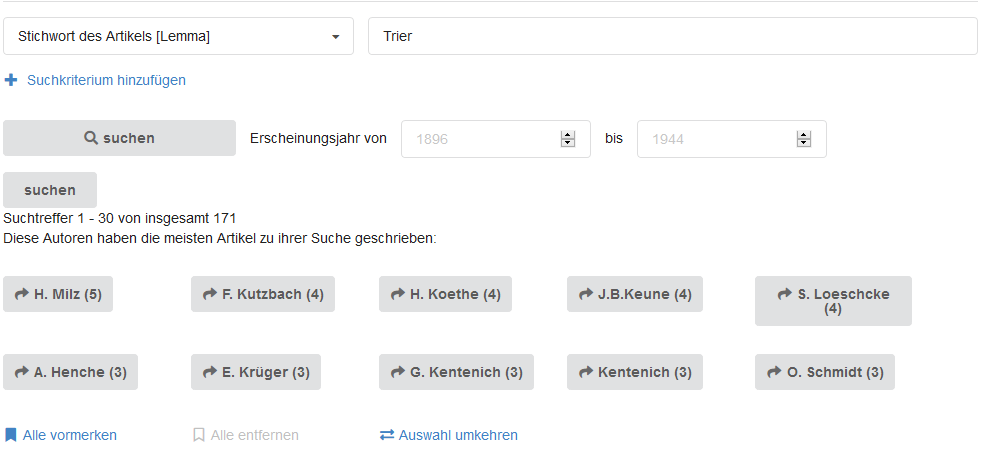
\includegraphics[width=1\linewidth]{images/best_authors.png}
	\caption{Abbildung der erweiterten Suche}
	\label{img:erweiterteSuche}
\end{figure}
